% \chapter{Client-server view (UML Component diagram)}\label{ch:client-server}


\begin{landscape}
    \section{Context diagram}
    The context diagram of the client-server view is displayed in figure \ref{fig:cc-context}. \\

    \centering
    \vspace*{\fill}

    \begin{figure}[!htp]
        \centering
        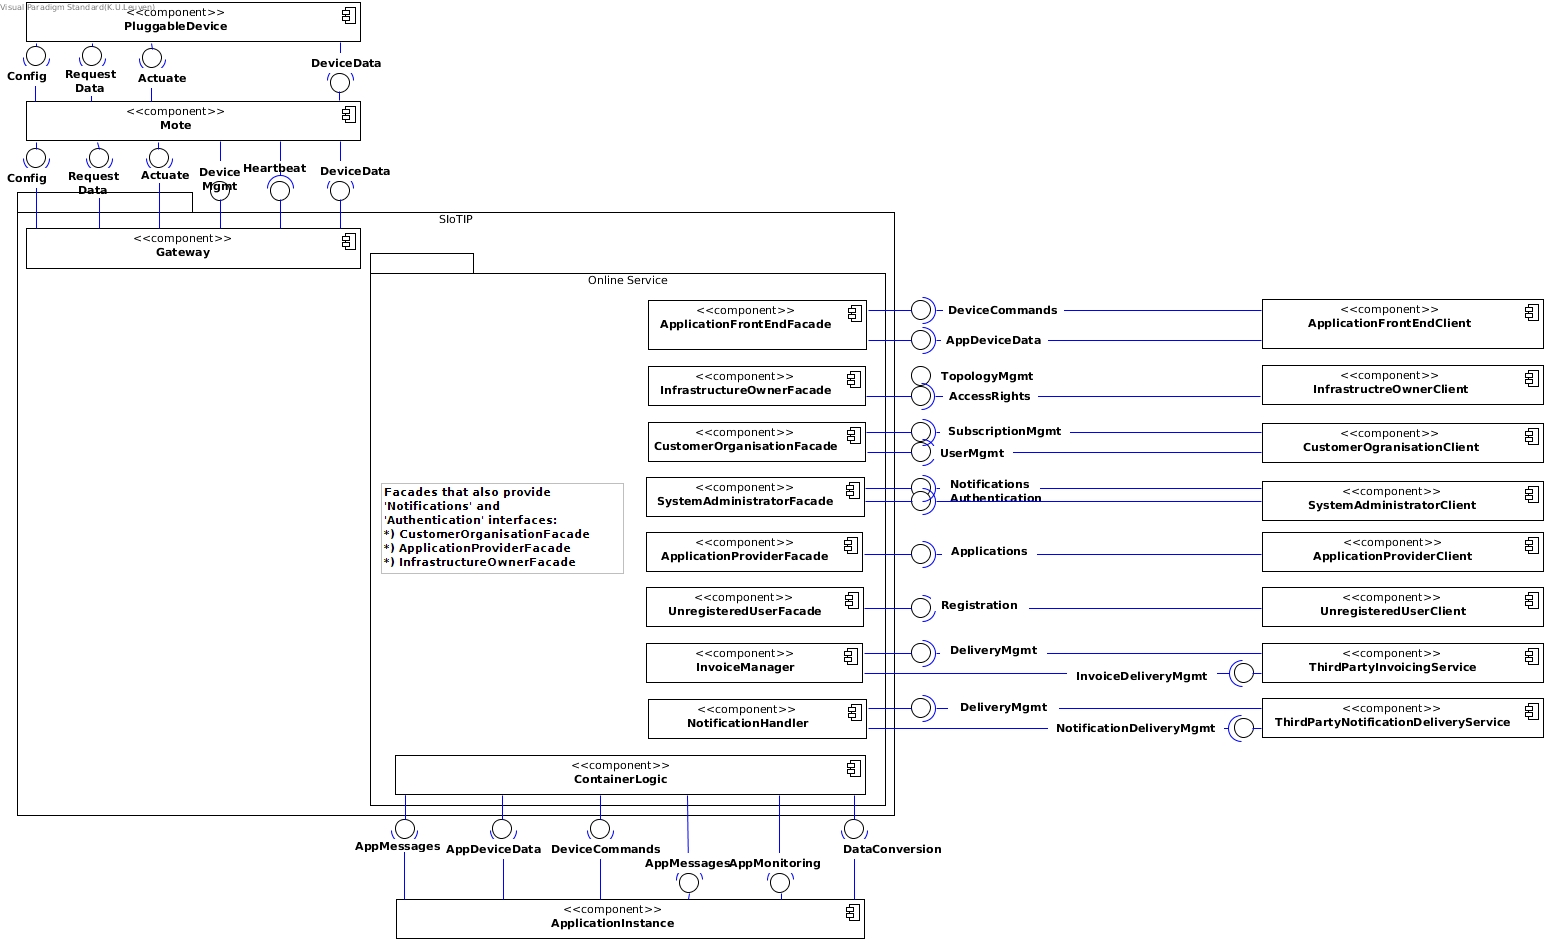
\includegraphics[width=\linewidth]{images/component-CONTEXT}
        \caption{Context diagram for the client-server view.}\label{fig:cc-context}
    \end{figure}

    \vfill
\end{landscape}


\begin{landscape}
    \section{Primary diagram}
    The primary diagram of the client-server view is displayed in figure \ref{fig:cc-primary}. \\

    \centering
    \vspace*{\fill}

    \begin{figure}[!htp]
        \centering
        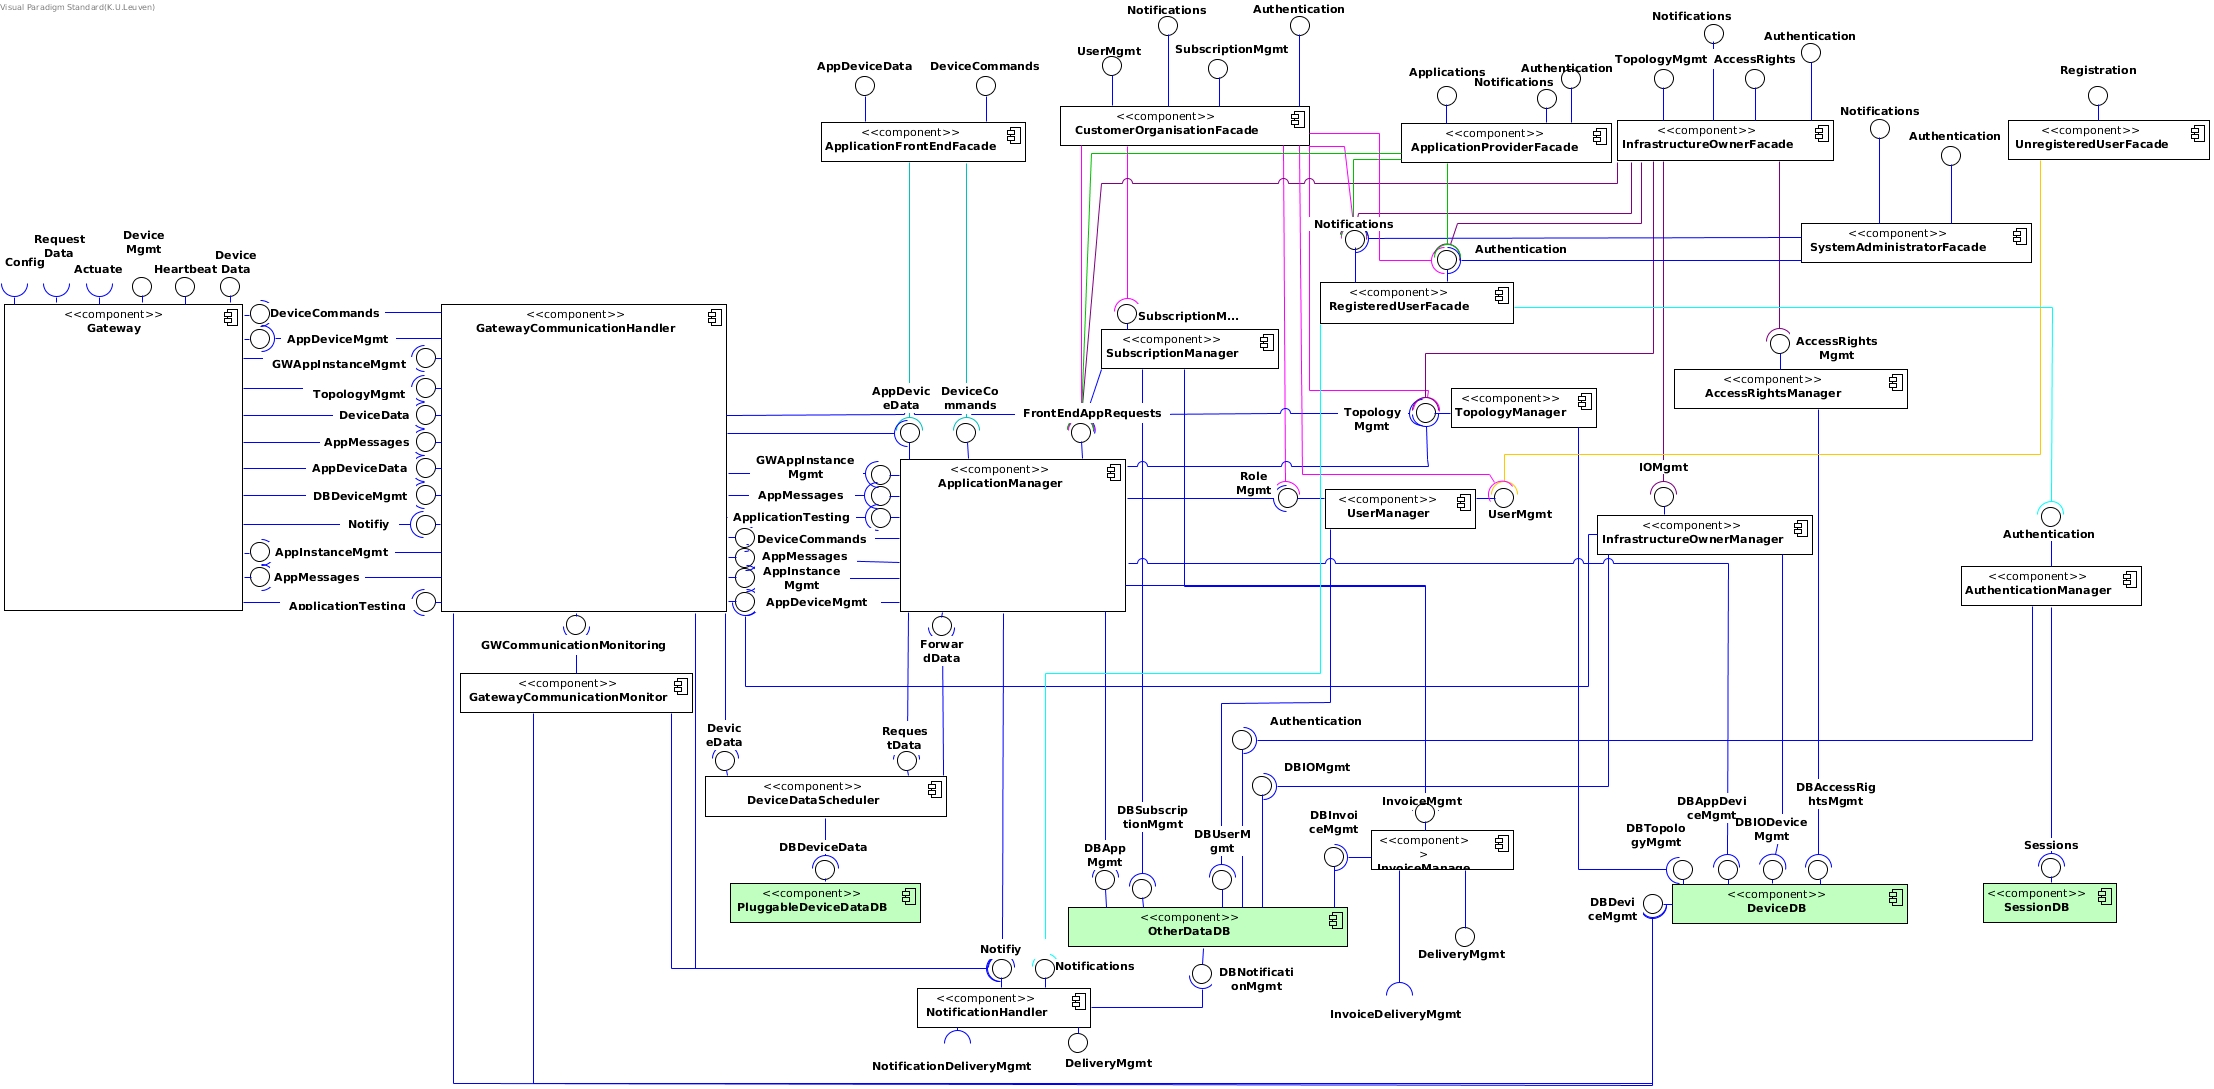
\includegraphics[width=\linewidth]{images/component-PRIMARY}
        \caption{Primary diagram of the client-server view.}\label{fig:cc-primary}
    \end{figure}

    \vfill
\end{landscape}
